\section{Context}
\subsection{Fault injection}

% FI
\begin{frame}[fragile]{Fault Injection}
\vfill
{
\small
\begin{columns}
    \begin{column}{0.4\textwidth}
     
        \vfill
        \textbf{Fault-injection attacks} %\cite{Boneh/EUROCRYPT97, Barenghi/IEEE2012}
        \begin{itemize}
            \item[]
            \item Lasers% \cite{Roscian/FDTC13, Colombier/HOST19}
            \item Electromagnetic pulses %\cite{Poucheret/FDTC11}
            \item Temperature %\cite{Hutter/ICSCRAA13}
            \item Power \& clock glitches% \cite{Schmidt/FDTC09, Yuce/HSS16}
            \item Software induced %\cite{Kim/ACM14, Seaborn/BH15}
            \item[]
        \end{itemize}
    
    \end{column}
    \begin{column}{0.6\textwidth}
        \only<1>{     
            \begin{figure}
                \centering
                \caption{Laser fault injection bench [1]}
                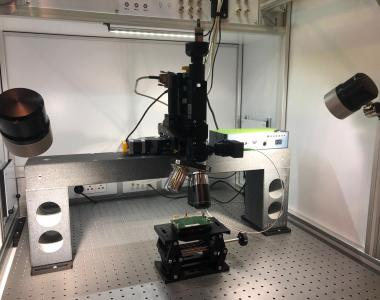
\includegraphics[width=0.67\textwidth]{img/s-lms4.jpg}
            \end{figure}
        }
        \only<2-> {
            \begin{figure}
                \centering
                \caption{Rowhammer principle [2]}
                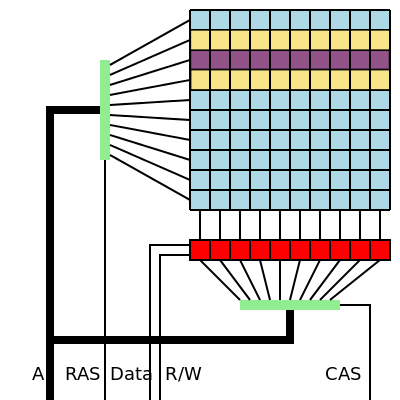
\includegraphics[width=0.55\textwidth]{img/Row_hammer.svg.png}
            \end{figure}
        }
    \end{column}
\end{columns}
\vfill
        \textit{Goal}: modify device behavior/state to break security property and gain advantage
}
\end{frame}

% Verify_pin
\begin{frame}[fragile]{\texttt{verify\_pin} program}
    \begin{columns}
        \begin{column}{0.55\textwidth}
            \begin{small}
                PIN verification program from FISSC \cite{Dureuil/PPLCC16} collection                
            \end{small}
            
            \vspace{0.2cm}
            
            \lstset{style=customc}
            \begin{lstlisting}
bool compare(uchar* a1, uchar* a2, size_t size)
{
    bool ret = true;
    size_t i = 0; 
    for(; i < size; i++)
        if(a1[i] != a2[i])
            ret = false;
        
    return ret;
}

bool verify_pin(uchar* user_pin) {
    if(try_counter > 0)  
        if(compare(user_pin, card_pin, PIN_SIZE)) {
            // Authentication
            try_counter = 3;
            return true;
        } else {
            try_counter--;
            return false;
        }
    return false;
}
            \end{lstlisting}	
        	\vfill
        \end{column}
        \begin{column}{0.45\textwidth}
        	\begin{small}
                 \begin{itemize}
                     \item Compare user PIN against the card's one in constant time
                     \item[] 
                     \item \textit{Attack objective:} being authenticated with a false PIN
                     \item[]
                 \end{itemize}
    	    \end{small}
            \vfill
        \end{column}
    \end{columns}
\end{frame}

% Fault example
\begin{frame}[fragile]{Faults injection - Example on \texttt{verify\_pin}}
    \begin{columns}
        \begin{column}{0.55\textwidth}
            \begin{small}
                PIN verification program from FISSC \cite{Dureuil/PPLCC16} collection                
            \end{small}
            
            \vspace{0.2cm}
            
            \lstset{style=customc, escapeinside={(*}{*)}}
            \begin{lstlisting}
bool compare(uchar* a1, uchar* a2, size_t size)
{
    bool ret = true;
    size_t i = 0; 
    for(; (*{\color{red} i < size}*); i++) // Fault: avoid the loop
        if(a1[i] != a2[i])
            ret = false;
        
    return ret;
}

bool verify_pin(uchar* user_pin) {
    if(try_counter > 0)  
        if(compare(user_pin, card_pin, PIN_SIZE)) {
            // Authentication
            try_counter = 3;
            return true;
        } else {
            try_counter--;
            return false;
        }
    return false;
}
            \end{lstlisting}	
        	\vfill
        \end{column}
        \begin{column}{0.45\textwidth}
        	\begin{small}
                 \begin{itemize}
                     \item Fault model: modelisation of the faults to be injected
                     \item[] $\rightarrow$ ex: \textbf{Test inversion}: inverse the branch taken during conditional branching
                     \item[]
                 \end{itemize}
    	    \end{small}
            \vfill
        \end{column}
    \end{columns}
\end{frame}

% CM example 
\begin{frame}[fragile, noframenumbering]{Faults injection - Example on \texttt{verify\_pin}}
    \begin{columns}
        \begin{column}{0.55\textwidth}
            \begin{small}
                PIN verification program from FISSC \cite{Dureuil/PPLCC16} collection                
            \end{small}
            
            \vspace{0.2cm}
            
            \lstset{style=customc, escapeinside={(*}{*)}}
            \begin{lstlisting}
bool compare(uchar* a1, uchar* a2, size_t size)
{
    bool ret = true;
    size_t i = 0; 
    for(; (*{\color{red} i < size}*); i++) // Fault
        if(a1[i] != a2[i])
            ret = false;
            
    if(i != size) // Countermeasure
        killcard(); 
        
    return ret;
}

bool verify_pin(uchar* user_pin) {
    if(try_counter > 0)  
        if(compare(user_pin, card_pin, PIN_SIZE)) {
            // Authentication
            try_counter = 3;
            return true;
        } else {
            try_counter--;
            return false;
        }
    return false;
}
            \end{lstlisting}	
        	\vfill
        \end{column}
        \begin{column}{0.45\textwidth}
        	\begin{small}
                 \begin{itemize}
                     \item Fault model: modelisation of the faults to be injected
                     \item[] $\rightarrow$ ex: Test inversion: inverse the branch taken during conditional branching
                     \item[]
                     \item \textbf{Software countermeasures (program transformations) can be placed to protect against faults}
                     \item[]
                 \end{itemize}
    	    \end{small}
            \vfill
        \end{column}
    \end{columns}
\end{frame}

% CM attack
\begin{frame}[fragile, noframenumbering]{Faults injection - Example on \texttt{verify\_pin}}
    \begin{columns}
        \begin{column}{0.55\textwidth}
            \begin{small}
                PIN verification program from FISSC \cite{Dureuil/PPLCC16} collection                
            \end{small}
            \vspace{0.2cm}
            
            \lstset{style=customc, escapeinside={(*}{*)}}
            \begin{lstlisting}
bool compare(uchar* a1, uchar* a2, size_t size)
{
    bool ret = true;
    size_t i = 0; 
    for(; (*{\color{red} i < size}*); i++) // Fault 1
        if(a1[i] != a2[i])
            ret = false;
            
    if((*{\color{red} i != size}*)) // Fault 2 => countermeasure attack
        killcard(); 
        
    return ret;
}

bool verify_pin(uchar* user_pin) {
    if(try_counter > 0)  
        if(compare(user_pin, card_pin, PIN_SIZE)) {
            // Authentication
            try_counter = 3;
            return true;
        } else {
            try_counter--;
            return false;
        }
    return false;
}
            \end{lstlisting}	
        	\vfill
        \end{column}
        \begin{column}{0.45\textwidth}
        	\begin{small}
                 \begin{itemize}
                     \item Fault model: modelisation of the faults to be injected
                     \item[] $\rightarrow$ ex: Test inversion: inverse the branch taken during conditional branching
                     \item[]
                     \item Software countermeasures (program transformations) can be placed to protect against faults
                     \item[] \textbf{multiples faults $\rightarrow$ countermeasures themselves can be attacked }
                     \item[]
                 \end{itemize}
    	    \end{small}
            \vfill
        \end{column}
    \end{columns}
\end{frame}


\subsection{Multiple faults}

\begin{frame}[fragile]{Multiple Faults}
\vfill
    State of the art attacks combine several faults to achieve their goal. % \cite{kim2007fault, Natella/ACM16}
    %Wookey Attack [Wookey 22]: first fault invalidate countermeasures, second exploit a buffer overflow vulnerability.
    \vspace{0.2cm}
    Most robustness evaluation tools consider only single fault
    
    {\small    
        \vspace{0.3cm}
        \
        \begin{itemize}
            \item Need to help developer and auditor in multiple faults
            \item []
            \item Standard analysis cannot be trivially applied
            \item[] $\rightarrow$ faults can induce modification in the CFG or the data flow
            \item []
            \item \onslide<2->{Exploration of faulted execution is subject to \textit{combinatory explosion} of paths due to faults}
            \item []
            \item []
        \end{itemize}
        
        \onslide<3->{    
            \begin{block}{\textbf{Probl. 1}}
                Need of automated tools to evaluate programs against multiple faults attacks
            \end{block}
        }
    }
\end{frame}


%%%%%%%%%%%%%%%%%%%%%%%%%%%%%%%%%%%%%%%%%%%%%%%%%%%%%%%%%%%%%%%%%%%%%%%%
\begin{frame}[fragile] \frametitle{Robustness evaluation in multiple faults} 
    \begin{small}
        \begin{itemize}
            \item Comparing the robustness of different protected versions of a program is not trivial
            \item [] $\Rightarrow$ \textit{attack surface paradox [Dureuil 2016]}: countermeasure can add attack surface to the code
            \item [] 
            \item How to count attacks in case of multiple faults ?
            \onslide<2-> {\item [] $\Rightarrow$ Which program is the most secure ?}
        \end{itemize}

        \begin{tiny}
            \centering
            \only<2>{
                \begin{table}[htb]
                    \setlength\tabcolsep{4pt}
                    \begin{tabular}{|l|l|c|c|c|c|c|c|c|}
                        \hline
                        \texttt{verify\_pin} version (from FISSC \cite{Dureuil/PPLCC16}) & countermeasures & 0-faults & 1-fault & 2-faults & 3-faults & 4-faults \\
                        \hline
                        vp\_0  \hfil & $\emptyset$ \hfil & 0     & 3 & 0  & 0  & 1 \\
                        \hline
                        vp\_1  \hfil & HB \hfil & 0     & 2 & 0  & 0  & 1 \\
                        \hline
                        vp\_2  \hfil & HB+FTL\hfil & 0     & 2 & 1  & 0  & 1 \\
                        \hline
                        vp\_3 \hfil &  HB+FTL+INL\hfil & 0     & 2 & 1  & 0  & 1 \\
                        \hline
                        vp\_4  \hfil & FTL+INL+DPTC+PTCBK+LC\hfil & 0     & 2 & 0  & 1  & 1 \\
                        \hline
                        vp\_5  \hfil & HB+FTL+DPTC+DC\hfil & 0     & 0 & 4  & 4  & 1 \\
                        \hline
                        vp\_6  \hfil & HB+FTL+INL+DPTC+DT \hfil & 0     & 0 & 3  & 0  & 1 \\
                        \hline
                        vp\_7  \hfil & HB+FTL+INL+DPTC+DT+SC\hfil & 0     & 0 & 2  & 0  & 1 \\
                        \hline
                    \end{tabular}
                \end{table}
            }
            \only<3->{
                \begin{table}[htb]
                    \setlength\tabcolsep{4pt}
                    \begin{tabular}{|l|l|c|c|c|c|c|c|c|}
                        \hline
                        \texttt{verify\_pin} version (from FISSC \cite{Dureuil/PPLCC16}) & countermeasures & 0-faults & 1-fault & 2-faults & 3-faults & 4-faults \\
                        \hline
                        vp\_0  \hfil & $\emptyset$ \hfil & 0     & 3 & 0  & 0  & 1 \\
                        \hline
                        vp\_1  \hfil & HB \hfil & 0     & 2 & 0  & 0  & 1 \\
                        \hline
                        vp\_2  \hfil & HB+FTL\hfil & 0     & 2 & 1  & 0  & 1 \\
                        \hline
                        vp\_3 \hfil &  HB+FTL+INL\hfil & 0     & 2 & 1  & 0  & 1 \\
                        \hline
                        \textbf{vp\_4}  \hfil & FTL+INL+DPTC+PTCBK+LC\hfil & \textbf{0}     & \textbf{2} & \textbf{0}  & 1  & 1 \\
                        \hline
                        \textbf{vp\_5}  \hfil & HB+FTL+DPTC+DC\hfil & \textbf{0}     & \textbf{0} & \textbf{4}  & 4  & 1 \\
                        \hline
                        vp\_6  \hfil & HB+FTL+INL+DPTC+DT \hfil & 0     & 0 & 3  & 0  & 1 \\
                        \hline
                        vp\_7  \hfil & HB+FTL+INL+DPTC+DT+SC\hfil & 0     & 0 & 2  & 0  & 1 \\
                        \hline
                    \end{tabular}
                \end{table}
            }
            \onslide<2-> {
                Legend:
                \begin{columns}
                    \begin{column}{0.5\textwidth}
                        \begin{itemize}
                            \item HB: hardened booleans
                            \item FTL: fixed time loops
                            \item INL: inlined function
                            \item PTC: try counter decremented first
                            \item PTCBK: try counter backup
                        \end{itemize}  
                    \end{column}
                    \begin{column}{0.5\textwidth}
                        \begin{itemize}
                            \item DC: double call
                            \item LC: loop counter verification
                            \item SC: step counter
                            \item DT: double test
                            \item CFI: control flow integrity \cite{Lalande/ESORICS14}
                        \end{itemize}  
                    \end{column}
                \end{columns}  
            }
        \end{tiny}

        \onslide<4->{
        \begin{columns}
            \begin{column}{0.8\textwidth}
                \begin{block}{\textbf{Probl. 2}}
                    How to evaluate programs and countermeasures in multiple-fault context ?
                \end{block}
            \end{column}
        \end{columns}
        }
    
    \vfill
    \end{small}
\end{frame}

\begin{frame}[fragile]{Countermeasures evaluation challenge in multiple faults}
\vfill
    {\small
        \begin{itemize}
            \item Try-and-error approaches are unsuitable for multi-faults
            \item[] $\rightarrow$ countermeasures themselves can be attacked
            \item [] $\rightarrow$ brute-forcing all countermeasures combinations is unrealistic
        \end{itemize}
    
        \begin{block}{
            \textbf{Probl. 3}}
            How to help to place countermeasures and give guarantees on the protected program in multiple faults context ?
        \end{block}
    
        \onslide<2-> {    
            \begin{itemize}
            \item[]
                \item $\rightarrow$ most tools use systematic (everywhere) placement approach
            \end{itemize}
            
            \begin{block}{\textbf{Probl. 4}}
            How to ensure that all added countermeasures are necessary ?
            \end{block}
        }
    }
\end{frame}

\subsection{Contributions}

\begin{frame}[fragile]{Contributions of this Thesis}
\vfill
    \begin{small}
        \begin{columns}
            \begin{column}{0.5\textwidth}    
                \textbf{Contributions}:
                \begin{itemize}
                    \item[]
                    \item Extension of the tool Lazart and of robustness analysis for multiple faults
                    \item [] $\rightarrow$ Problematic \textit{P1}, \textit{P2}
                    \item[]
                    \item \onslide<2->{Isolation analysis and placement algorithms}
                    \item[] \onslide<2->{$\rightarrow$ Problematic \textit{P2}, \textit{P3}}
                    \item []
                    \item \onslide<3->{Optimization of detector-based countermeasures}
                    \item [] \onslide<3->{$\rightarrow$ Problematic \textit{P2}, \textit{P4}}
                    \item[] 
                \end{itemize}
                
                \vfill
            
            \end{column}
            \begin{column}{0.5\textwidth}
                \textbf{Problematics:}
                \begin{itemize}
                    \item  \textit{P1}: Multi-faults tools
                    \item  \textit{P2}: Countermeasures evaluation / comparison
                    \item  \textit{P3}: Countermeasures placement
                    \item  \textit{P4}: Countermeasures necessity
                    \item[] 
                \end{itemize}
                
            \end{column}
        \end{columns}        
    \end{small}
\end{frame}
